% Generated from draft.md by build_draft.py.
% ============================================================================
% DHG508 Final Design Paper & Post-Mortem (Overleaf Source)
% Lingnan University — Critical Digital History
%
% OVERLEAF SETUP:
%   1. Upload overleaf-final.zip (or overleaf-draft.zip) to Overleaf
%   2. Menu (top left) -> Compiler -> XeLaTeX
%   3. Click Recompile
% ============================================================================

\documentclass[11pt,a4paper]{article}

\usepackage{fontspec}
\IfFontExistsTF{Times New Roman}
  {\setmainfont{Times New Roman}}
  {\setmainfont{texgyretermes}[Extension=.otf,UprightFont=*-regular,BoldFont=*-bold,ItalicFont=*-italic,BoldItalicFont=*-bolditalic]}

\usepackage{xeCJK}
\IfFontExistsTF{Noto Serif CJK SC}
  {\setCJKmainfont{Noto Serif CJK SC}\setCJKmonofont{Noto Serif CJK SC}}
  {\IfFontExistsTF{Songti SC}
    {\setCJKmainfont{Songti SC}\setCJKmonofont{Songti SC}}
    {\IfFontExistsTF{SimSun}
      {\setCJKmainfont{SimSun}\setCJKmonofont{SimSun}}
      {\setCJKmainfont{FandolSong-Regular.otf}\setCJKmonofont{FandolSong-Regular.otf}}}}

\usepackage[a4paper, margin=0.8in]{geometry}
\usepackage{setspace}
\usepackage{booktabs}
\usepackage{array}
\usepackage{graphicx}
\usepackage{csquotes}
\usepackage{microtype}

% Chicago Manual of Style 18th ed., Notes-Bibliography (BibLaTeX + Biber)
\usepackage[notes, backend=biber, autolang=other, isbn=false]{biblatex-chicago}
\addbibresource{references.bib}

\renewcommand{\footnotesize}{\fontsize{9}{11}\selectfont}
\usepackage{xurl}
\usepackage[hidelinks]{hyperref}
\setlength{\emergencystretch}{2.5em}
\setlength{\parskip}{0.14em}
\setstretch{1.01}

\title{\textbf{Playing with Uncertain Provenance}\\[0.25em]
\large Evidence Boundaries, Deterministic Rehearsal, and the Design of \emph{Thief Simulator}}
\author{Yutong Li\\Lingnan University $\cdot$ DHG508 Critical Digital History\\
\small Release Build: \texttt{v0.26.16} (Desktop Windows / Linux / macOS) $\cdot$ Repo: \url{https://github.com/Olipias/thief-sim}}
\date{25 November 2026}

\begin{document}
\maketitle
\begin{abstract}
\noindent
\emph{Thief Simulator} is a Chinese-language 2D stealth and investigation game built in Godot 4.7 for desktop. You examine museum objects whose identifications are secure while their ownership histories are not, rehearse heist routes in a deterministic simulation, and decide whether to hand a relic to a demon contract or to a national receiver. Every claim carries a label: documented fact (据), scholarly inference (推断), or design invention (设). This paper describes the build and what testing exposed.
\end{abstract}
\section{Historical Question and Medium}
A museum label can pin down an object while leaving its movement between owners blank. The game asks what a player can conclude when records fix an artifact's form and acquisition date but say nothing about how it left its place of origin. A heist needs a target in a display case; provenance research meets missing transfers and unverified rumors. Both pressures stay visible.

The audience is Chinese-reading players who like short stealth games. You answer four questions about a relic: how it looks, where it came from, how it entered a collection, and which gallery holds it tonight. One answer leaves the rest open. Casting seams identify a Shang bronze; they do not explain its route out of China before the 1930s.

Interactivity turns that distinction into a task. After a six-panel comic and a tutorial heist, you enter a walkable safehouse. At the computer you search catalog numbers, drag source cards into an evidence frame, and pick the claim they support. The phone and door stay locked until you verify one relic's features and exhibition zone. In the museum you scout rooms, lift ordinary loot, and leave without the main relic.

\section{Sources and Scholarly Conversation}
The investigation rests on three real antiquities. The Metropolitan Museum of Art catalogs heart scarab \texttt{10.130.1650} as a Late Period (664--332 BCE) dark green stone amulet given in 1910.\autocite[Artwork Details]{met} That record confirms material and arrival in New York, not an excavation or an export from Egypt. UNESCO lists painted askos \texttt{VM-GR-25-012} from the West House at Akrotiri as a Late Cycladic I (1650--1615 BCE) vessel, with no theft date and no current location.\autocite[About the object]{unesco} The \emph{West House} card tests whether players separate an ancient building from the museum's modern west wing.

Adam Chapman argues that historical games carry meaning through rules and the actions they ask of players, not through text alone.\autocite[opening discussion]{chapman2012} An early build let one button connect clue cards. His argument named the problem, since accurate prose does nothing when the player performs no analysis. I rebuilt the computer board (\texttt{investigation\_\allowbreak{}board.gd}) around manual work: confirming the double-ram \emph{zun} takes two cards and a chosen relation between its twin-ram body and pre-cast horns.

Jeremiah McCall treats historical simulations as problem spaces, where goals, resources, and affordances organize what a player can do.\autocite[part I]{mccall2012} That framing exposed a conflict between stealth rewards and historical care. Price every artifact and the economy teaches players to treat antiquities as cargo. I split objects in \texttt{game\_\allowbreak{}state.gd} into two classes: ordinary loot passes through a box, a phone reservation, and a front-door sale, while the three principal relics reach only the demon or national-receiver endings.

Quanyu Wang and Sascha Priewe supply the technical basis for British Museum double-ram \emph{zun} \texttt{1936,1118.1}. Their metallurgical study shows horns cast separately and locked onto the body, and links the vessel's style to a southern bronze tradition in the middle Yangtze region.\autocite[257--58, 266, 273]{wang2013} They record a 1930s Eumorfopoulos entry with no known findspot. The museum's catalog page returned HTTP 403 in November 2026, so I worked from their text and our earlier log, and removed an unverified 1860 looting rumor from \texttt{story.gd}.

\section{Architecture and Boundaries}
The game runs at 640 by 360 on Godot 4.7, exporting through \texttt{tools/\allowbreak{}export.sh}. The controller in \texttt{src/\allowbreak{}main.gd} moves between the comic, the tutorial gallery, the safehouse (\texttt{safehouse.gd}), and the museum (\texttt{museum.gd}). Four stations organize the routine: computer, storage box, phone, and door.

Figure 1 traces data from sources through the controller, saves, simulation, and tests. Fact IDs (\texttt{C-001} to \texttt{C-003}) live in \texttt{investigation.gd} and \texttt{story.gd}, apart from \texttt{user:/\allowbreak{}/\allowbreak{}save.json}. On a retry, \texttt{GameState} keeps discovery (\texttt{story\_\allowbreak{}flags}) separate from the physical snapshot, so detection rewinds position and spent items while uncovered rooms stay uncovered.

Rehearsal and execution share one fixed-tick kernel (\texttt{sim\_\allowbreak{}preview.gd}, 20 ticks per second). Tab or R freezes player, patrols, cameras, and noise decay together through \texttt{\_\allowbreak{}sync\_\allowbreak{}world\_\allowbreak{}freeze}. The kernel simulates a copy of the room for predicted paths and warnings, then Space runs the plan through the same tick function.

Documented history stops at 1936 for the \emph{zun}, 1910 for the scarab, and the Bronze Age eruption at Akrotiri. Contemporary elements are invention: three relics in one museum, exhibition slips, guard routes, and the demon. Citations sit in the title declaration while the board enforces the limits.

\begin{figure}[!htbp]
  \centering
  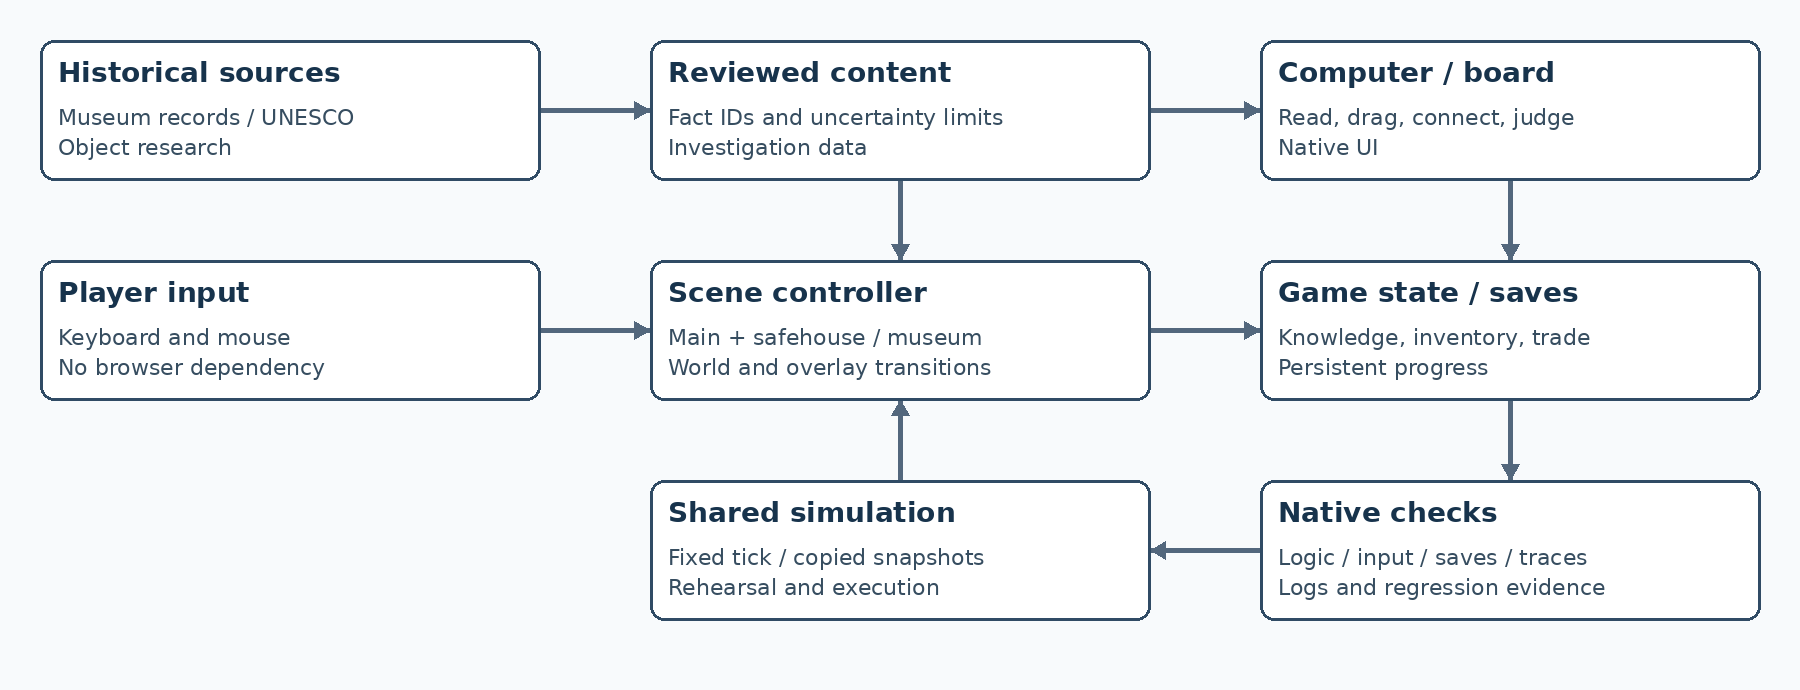
\includegraphics[width=0.92\textwidth]{schematic.png}
  \caption{Source review, scene control, deterministic simulation, and native verification modules.}
  \label{fig:schematic}
\end{figure}

\section{Evidence Table}
Table 1 maps seven claims and mechanics from \texttt{paper/\allowbreak{}evidence.csv}, generated by \texttt{make\_\allowbreak{}evidence\_\allowbreak{}table.py}. Labels attach to single claims: Wang and Priewe support an observation on page 266 and an attribution on page 273.

\begin{table}[!htbp]
  \centering
  \scriptsize
  \setlength{\tabcolsep}{3.5pt}
  \renewcommand{\arraystretch}{1.22}
  % Auto-generated from evidence.csv by make_evidence_table.py — edit the CSV, not this file.
\begin{tabular}{p{0.27\textwidth}p{0.20\textwidth}p{0.13\textwidth}p{0.08\textwidth}p{0.22\textwidth}}
  \toprule
  \textbf{Claim / Element} & \textbf{Source / File} & \textbf{Locator} & \textbf{Level} & \textbf{Boundary / Limit} \\
  \midrule
  The double-ram zun has separately cast horns attached by lock-on casting. & Wang and Priewe 2013 & p. 266 & 据 & Does not establish a complete ownership history before 1936. \\
  The double-ram zun belongs to a southern Chinese bronze tradition. & Wang and Priewe 2013 & p. 273 & 推断 & Does not prove a specific excavated findspot in Hunan. \\
  Heart scarab 10.130.1650 is dark green stone donated in 1910. & Met object 10.130.1650 & Artwork Details & 据 & Does not document earlier excavation or export from Egypt. \\
  Painted askos VM-GR-25-012 comes from the West House at Akrotiri. & UNESCO VM-GR-25-012 & About the object & 据 & The ancient West House is an archaeological building rather than a modern museum wing. \\
  Three principal relics appear in one mission museum. & src/data/investigation.gd & Story scenario & 设 & Fictional temporary display rather than real simultaneous exhibition. \\
  A demon contract motivates the protagonist and frames delivery choices. & src/data/story.gd & Opening CG \& ending branches & 设 & Fictional narrative premise rather than historical or legal authority. \\
  Rehearsal and execution traces match tick by tick on identical snapshots. & tests/test\_museum\_sim.gd & 52-check museum sim suite & 据 & Covers deterministic stealth rules rather than historical museum operations. \\
  \bottomrule
\end{tabular}

  \caption{Claims and design elements with locators, evidence tiers (据 documented, 推断 inferred, 设 invented), and limits.}
  \label{tab:evidence}
\end{table}

\section{Verification and Playtesting}
\texttt{tools/\allowbreak{}verify.sh --visual} runs 25 stages. Build \texttt{v0.26.16} passed all 25 and 56 visual comparisons on 25 November 2026.

\begin{enumerate}
  \item \textbf{Logic and history:} \texttt{test\_\allowbreak{}logic.gd} (2,552 assertions) and \texttt{test\_\allowbreak{}history.py} (11) hold the four evidence tiers and reject the 1860 rumor.
  \item \textbf{Simulation:} \texttt{test\_\allowbreak{}sim\_\allowbreak{}preview.gd} and \texttt{test\_\allowbreak{}museum\_\allowbreak{}sim.gd} (133) compare rehearsal and execution tick by tick and confirm a rewind restores coordinates without touching the wallet.
  \item \textbf{Input and layout:} \texttt{test\_\allowbreak{}input\_\allowbreak{}flow.gd} and \texttt{test\_\allowbreak{}dialogue\_\allowbreak{}paging.gd} (563) drive key and mouse events through search, dragging, departure gates, and pagination at 640 by 360.
  \item \textbf{Economy and saves:} \texttt{test\_\allowbreak{}safehouse\_\allowbreak{}loop.gd} (33) runs loot through delivery and purchase; \texttt{test\_\allowbreak{}save\_\allowbreak{}compat.gd} (135) covers damaged saves.
\end{enumerate}

Playtesting caught four defects unit tests missed: guards frozen while the player moved during takeover (\texttt{v0.23.3}), a board with no next step (\texttt{v0.26.14}), one contact introduction reused for six people (\texttt{v0.26.13}), and labels overflowing the dialogue box (\texttt{v0.26.15}). Each fix carries a regression test.

\section{Post-Mortem}
\textbf{What worked.} Fact IDs kept dialogue honest, since \texttt{test\_\allowbreak{}history.py} catches sentences that turn an inference into a findspot. Separating stock (\texttt{smoke\_\allowbreak{}stock}) from carried gear (\texttt{smoke\_\allowbreak{}count}) closed a duplication path during rewinds.

\textbf{What failed.} Early tests compared the shared prefix of two traces and polled once per frame, so preview ticks that ran past the route's end went unnoticed. \texttt{v0.26.9} stops rehearsal at the final waypoint and emits per-tick signals. UI tests that called \texttt{open()} and \texttt{close()} directly hid input bleed-through; real \texttt{InputEvent} dispatches exposed it.

\textbf{What changed.} I cut the artifact-spirit dialogues (\texttt{v0.20.0}), dropped the closing countdown (\texttt{v0.21.4}), limited fog to the minimap (\texttt{v0.26.12}), and replaced the three-chain requirement with one verified target.

\textbf{Where the build falls short.} This release is a working prototype, not the game I set out to make. Most rooms still carry placeholder pixel art, the dialogue reads as a draft script rather than finished writing, and audio stops at procedurally generated cues with no music or mixing pass. Development halted when the AI tooling budget ran out, which froze the build at this state. The systems, the evidence boundaries, and the tests hold up under review; the presentation does not yet.

\textbf{Limits and AI assistance.} Automated suites and the Linux boot pass on \texttt{v0.26.16}; Windows and macOS host testing and a player study remain open. I designed the mechanics, set the historical boundaries, wrote the paper, and verified every citation myself. AI tools assisted with implementation: OpenCode, Codex, and Claude Code for GDScript debugging and test scaffolding, Tencent Hunyuan3D for sprite rendering, and \texttt{stop-slop} with \texttt{Humanizer-zh} for English style.
\singlespacing
\printbibliography[title={Bibliography}]

\end{document}
